\documentclass[tikz,border=10pt]{standalone}
% Shared look for every TikZ diagram. Load with % Shared look for every TikZ diagram. Load with % Shared look for every TikZ diagram. Load with \input{../../tools/tikz-style.tex}
\usepackage[T1]{fontenc}
\usepackage{lmodern}
\renewcommand{\sfdefault}{lmr}  % diagrams use the same serif as the text
\usetikzlibrary{arrows.meta, positioning, shapes.geometric, calc, fit, backgrounds}
\definecolor{cblue}{HTML}{4C78A8}
\definecolor{corange}{HTML}{F58518}
\definecolor{cgreen}{HTML}{54A24B}
\definecolor{cred}{HTML}{E45756}
\definecolor{cpurple}{HTML}{B279A2}
\definecolor{cgrey}{HTML}{6B6B6B}
\tikzset{
  every picture/.style={font=\sffamily, line width=1.2pt},
  box/.style={draw=#1, fill=#1!12, rounded corners=4pt, align=center, inner sep=7pt, minimum height=1.1cm},
  box/.default=cgrey,
  arrow/.style={-{Stealth[length=3mm]}, draw=cgrey, line width=1.4pt},
  title/.style={font=\sffamily\bfseries\Large},
  note/.style={font=\sffamily\small, text=cgrey, align=center},
}
\AtBeginDocument{\hyphenpenalty=10000 \exhyphenpenalty=10000}

\usepackage[T1]{fontenc}
\usepackage{lmodern}
\renewcommand{\sfdefault}{lmr}  % diagrams use the same serif as the text
\usetikzlibrary{arrows.meta, positioning, shapes.geometric, calc, fit, backgrounds}
\definecolor{cblue}{HTML}{4C78A8}
\definecolor{corange}{HTML}{F58518}
\definecolor{cgreen}{HTML}{54A24B}
\definecolor{cred}{HTML}{E45756}
\definecolor{cpurple}{HTML}{B279A2}
\definecolor{cgrey}{HTML}{6B6B6B}
\tikzset{
  every picture/.style={font=\sffamily, line width=1.2pt},
  box/.style={draw=#1, fill=#1!12, rounded corners=4pt, align=center, inner sep=7pt, minimum height=1.1cm},
  box/.default=cgrey,
  arrow/.style={-{Stealth[length=3mm]}, draw=cgrey, line width=1.4pt},
  title/.style={font=\sffamily\bfseries\Large},
  note/.style={font=\sffamily\small, text=cgrey, align=center},
}
\AtBeginDocument{\hyphenpenalty=10000 \exhyphenpenalty=10000}

\usepackage[T1]{fontenc}
\usepackage{lmodern}
\renewcommand{\sfdefault}{lmr}  % diagrams use the same serif as the text
\usetikzlibrary{arrows.meta, positioning, shapes.geometric, calc, fit, backgrounds}
\definecolor{cblue}{HTML}{4C78A8}
\definecolor{corange}{HTML}{F58518}
\definecolor{cgreen}{HTML}{54A24B}
\definecolor{cred}{HTML}{E45756}
\definecolor{cpurple}{HTML}{B279A2}
\definecolor{cgrey}{HTML}{6B6B6B}
\tikzset{
  every picture/.style={font=\sffamily, line width=1.2pt},
  box/.style={draw=#1, fill=#1!12, rounded corners=4pt, align=center, inner sep=7pt, minimum height=1.1cm},
  box/.default=cgrey,
  arrow/.style={-{Stealth[length=3mm]}, draw=cgrey, line width=1.4pt},
  title/.style={font=\sffamily\bfseries\Large},
  note/.style={font=\sffamily\small, text=cgrey, align=center},
}
\AtBeginDocument{\hyphenpenalty=10000 \exhyphenpenalty=10000}

\begin{document}
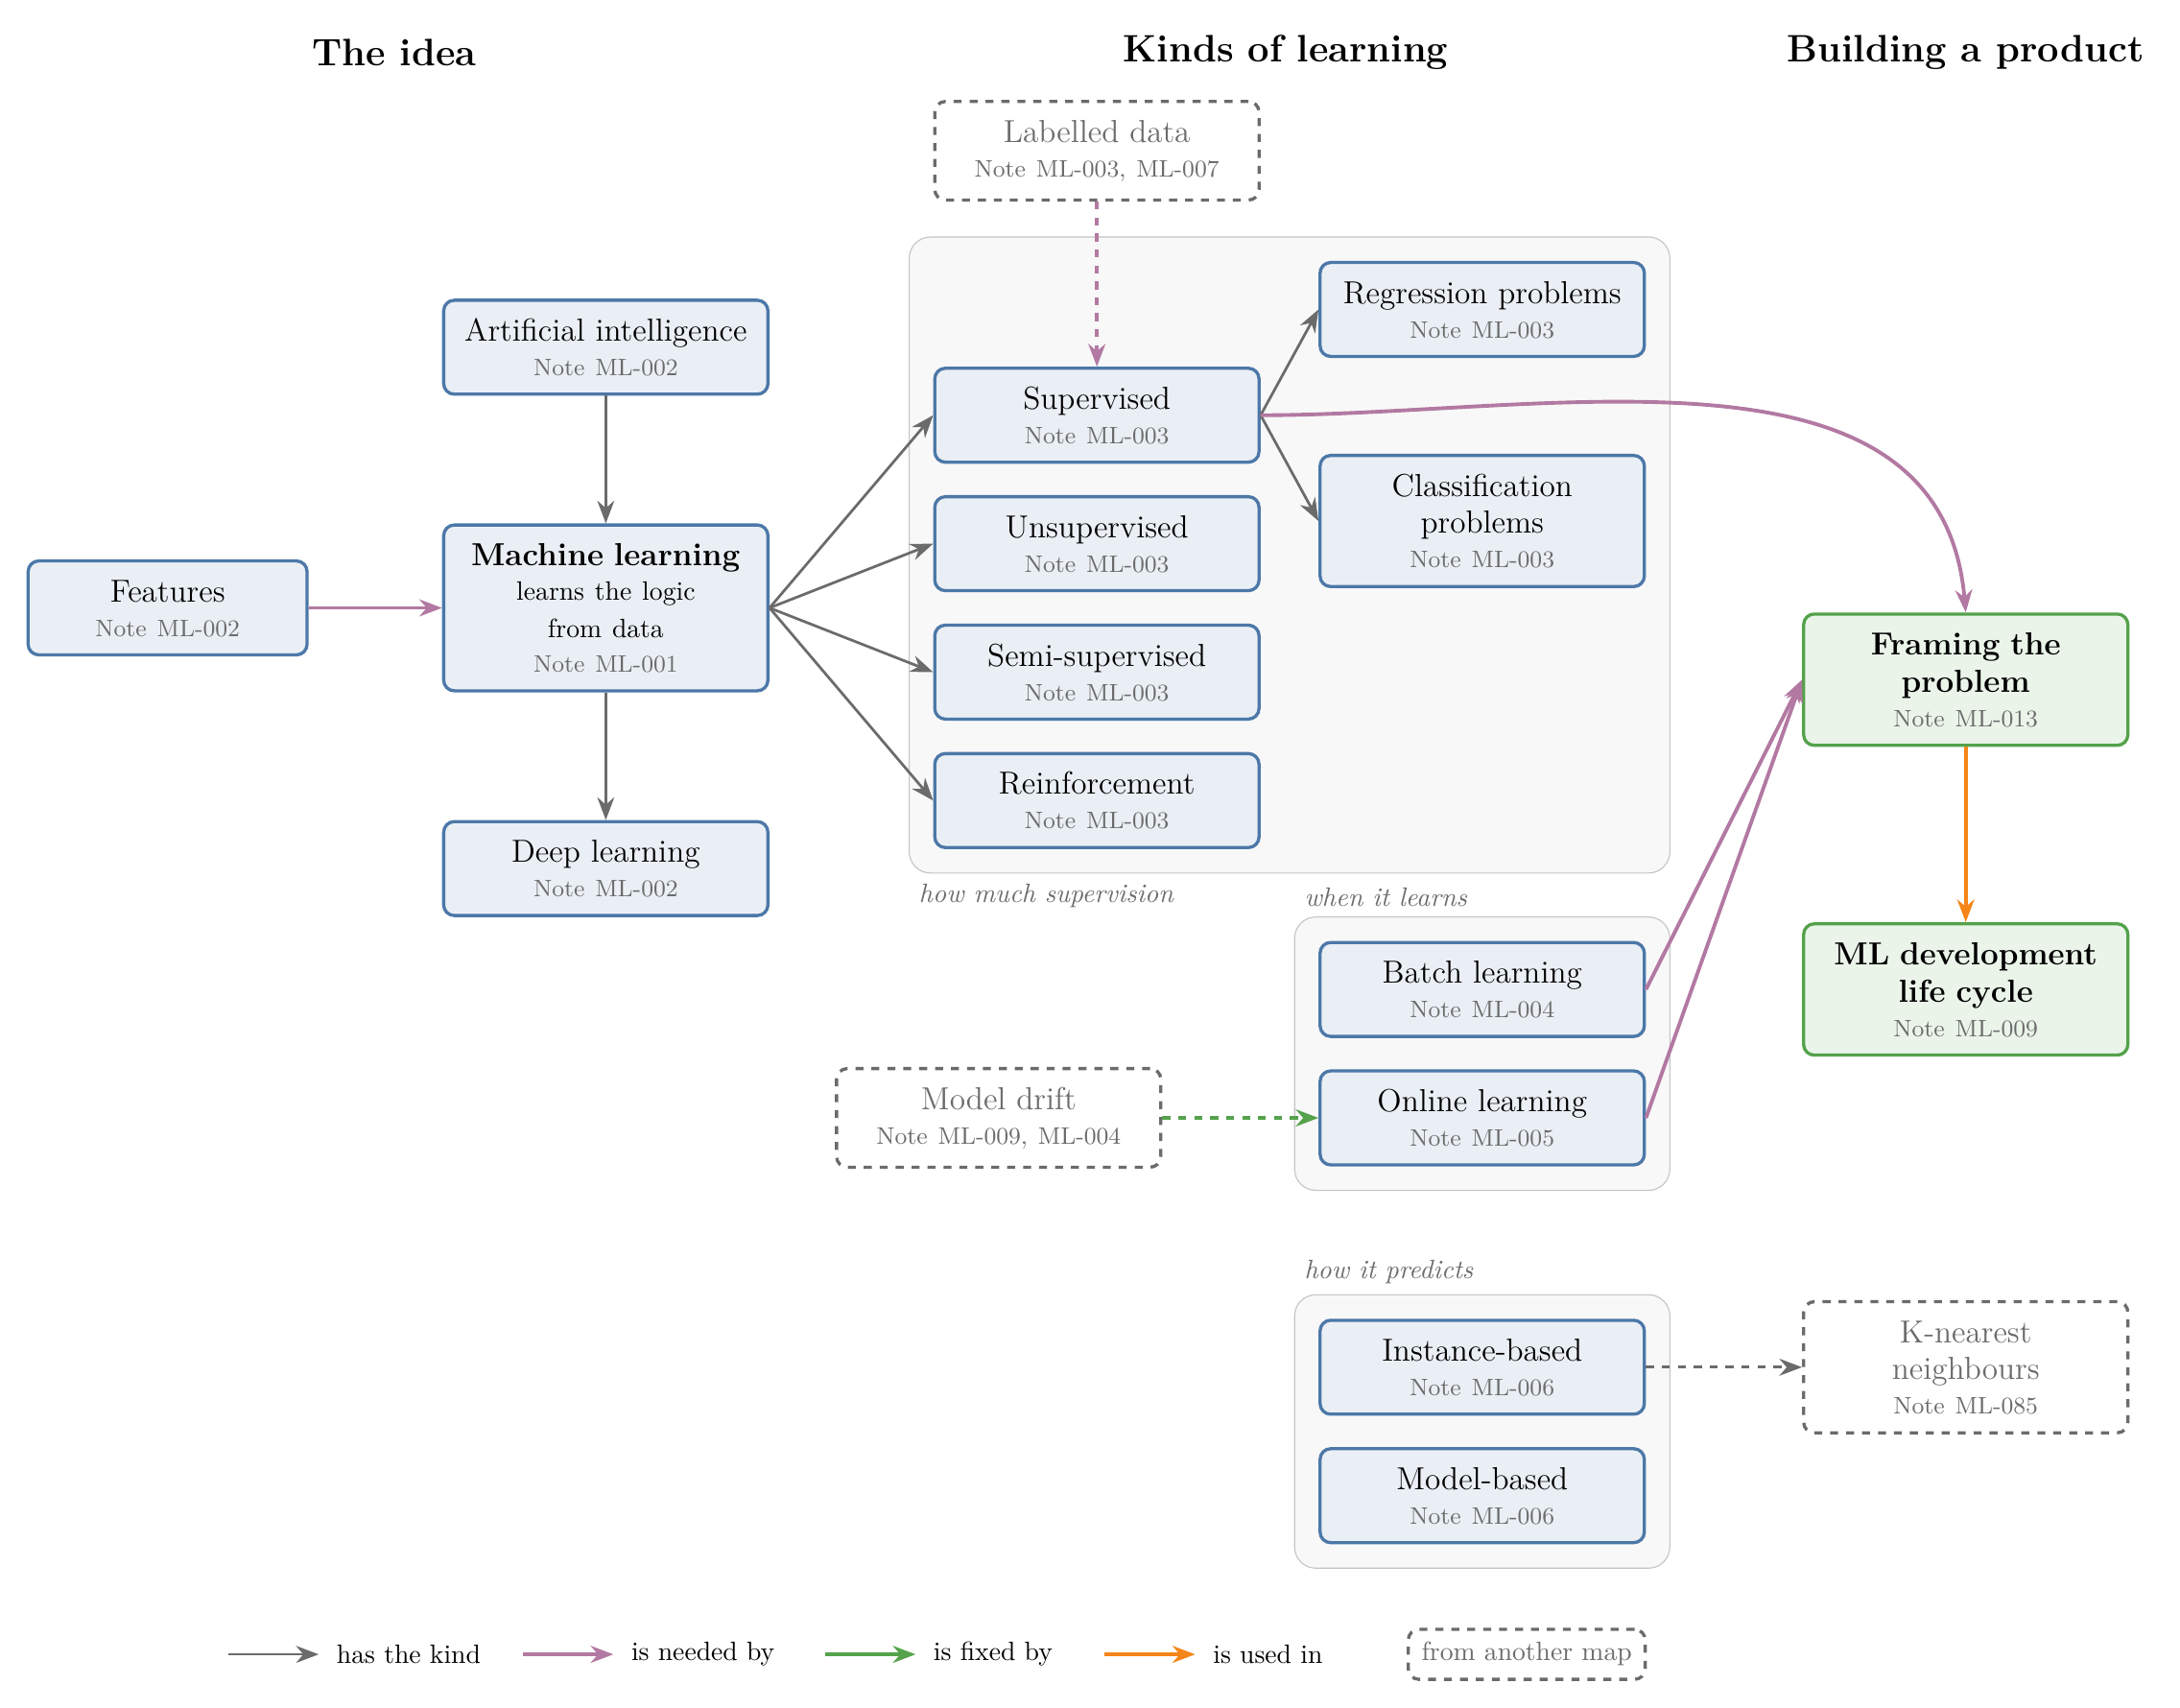
\begin{tikzpicture}[
    every node/.append style={font=\sffamily\large},
    idea/.style={box=cblue, text width=3.8cm},
    kind/.style={box=cblue, text width=3.8cm},
    build/.style={box=cgreen, text width=3.8cm},
    probl/.style={box=cred, text width=3.8cm},
    prev/.style={draw=cgrey, dashed, rounded corners=4pt, align=center, inner sep=7pt, text=cgrey, text width=3.8cm, minimum height=1.1cm},
    group/.style={draw=cgrey!40, fill=cgrey!5, rounded corners=8pt, inner sep=9pt},
    gname/.style={font=\sffamily\normalsize\itshape, text=cgrey, anchor=south west},
    kindof/.style={arrow, draw=cgrey, line width=1pt},
    needs/.style={arrow, draw=cpurple},
    fixes/.style={arrow, draw=cgreen},
    usedin/.style={arrow, draw=corange},
  ]
  \newcommand{\nt}[1]{\\[-1pt]{\small\color{cgrey}Note #1}}
  \node[title] at (-2.8,13.8) {The idea};
  \node[title] at (9,13.8) {Kinds of learning};
  \node[title] at (18,13.8) {Building a product};

  % the idea
  \node[idea] (ai) at (0,9.9)  {Artificial intelligence\nt{ML-002}};
  \node[idea] (ml) at (0,6.45) {\textbf{Machine learning}\\[-1pt]{\normalsize learns the logic from data}\nt{ML-001}};
  \node[idea] (dl) at (0,3.0)  {Deep learning\nt{ML-002}};
  \node[idea, text width=3.2cm] (feat) at (-5.8,6.45) {Features\nt{ML-002}};
  \draw[kindof] (ai) -- (ml);
  \draw[kindof] (ml) -- (dl);
  \draw[needs] (feat) -- (ml);

  % kinds: how much supervision
  \node[kind] (sup)   at (6.5,9.0) {Supervised\nt{ML-003}};
  \node[kind] (unsup) at (6.5,7.3) {Unsupervised\nt{ML-003}};
  \node[kind] (semi)  at (6.5,5.6) {Semi-supervised\nt{ML-003}};
  \node[kind] (rein)  at (6.5,3.9) {Reinforcement\nt{ML-003}};
  \node[kind] (reg)   at (11.6,10.4) {Regression problems\nt{ML-003}};
  \node[kind] (cls)   at (11.6,7.6)  {Classification problems\nt{ML-003}};
  \node[prev] (lab)   at (6.5,12.5) {Labelled data\nt{ML-003, ML-007}};
  % kinds: when it learns
  \node[kind] (batch)  at (11.6,1.4)  {Batch learning\nt{ML-004}};
  \node[kind] (online) at (11.6,-0.3) {Online learning\nt{ML-005}};
  \node[prev] (drift)  at (5.2,-0.3)  {Model drift\nt{ML-009, ML-004}};
  % kinds: how it predicts
  \node[kind] (inst)  at (11.6,-3.6) {Instance-based\nt{ML-006}};
  \node[kind] (model) at (11.6,-5.3) {Model-based\nt{ML-006}};
  \node[prev] (knn)   at (18,-3.6)  {K-nearest neighbours\nt{ML-085}};

  \begin{scope}[on background layer]
    \node[group, fit=(sup) (rein) (reg) (cls)] (g1) {};
    \node[group, fit=(batch) (online)] (g2) {};
    \node[group, fit=(inst) (model)] (g3) {};
  \end{scope}
  \node[gname] at (g2.north west) {when it learns};
  \node[gname] at (g3.north west) {how it predicts};
  \node[gname, anchor=north west] at (g1.south west) {how much supervision};

  \foreach \k in {sup, unsup, semi, rein} \draw[kindof] (ml.east) -- (\k.west);
  \draw[kindof] (sup.east) -- (reg.west);
  \draw[kindof] (sup.east) -- (cls.west);
  \draw[needs, dashed] (lab) -- (sup);
  \draw[fixes, dashed] (drift) -- (online);
  \draw[kindof, dashed] (inst) -- (knn);

  % building a product
  \node[build] (frame) at (18,5.5) {\textbf{Framing the problem}\nt{ML-013}};
  \node[build, minimum height=1.6cm] (mldlc) at (18,1.4) {\textbf{ML development}\\\textbf{life cycle}\nt{ML-009}};
  \draw[needs] (sup.east) to[out=0, in=95] (frame.north);
  \draw[needs] (batch.east) -- (frame.west);
  \draw[needs] (online.east) -- (frame.west);
  \draw[usedin] (frame) -- (mldlc);

  % legend
  \begin{scope}[shift={(-5,-7.4)}, every node/.style={font=\sffamily, anchor=west}]
    \draw[kindof] (0,0) -- (1.2,0);   \node at (1.3,0) {has the kind};
    \draw[needs] (3.9,0) -- (5.1,0);  \node at (5.2,0) {is needed by};
    \draw[fixes] (7.9,0) -- (9.1,0);  \node at (9.2,0) {is fixed by};
    \draw[usedin] (11.6,0) -- (12.8,0); \node at (12.9,0) {is used in};
    \node[draw=cgrey, dashed, rounded corners=4pt, inner sep=5pt, text=cgrey, anchor=west] at (15.6,0) {from another map};
  \end{scope}
\end{tikzpicture}
\end{document}
